\textbf{\textit{``You can know the name of a bird in all the languages of the world, but when you're finished, you'll know absolutely nothing whatever about the bird... So let's look at the bird and see what it's doing -- that's what counts. I learned very early the difference between knowing the name of something and knowing something.''}}

Richard Feynman (1918 - 1988) 


\chapter{Data analysis}
\label{chap:dataanalysis}
\section{Overview}

The overall process of data analysis is not linear in DM and it requires experimentation to achieve useful insights. However, the process can be usefully considered as comprising three main steps: data extraction, transformation, and loading for analysis. 

In this case the subset of patient safety reports relating to computer problems extracted from the NRLS database using a SAS query were cleaned and quality checked before being explored, transformed, and loaded for further analysis, see figure \ref{fig:dataminingoverview}.

\begin{figure}[htp]
\centering
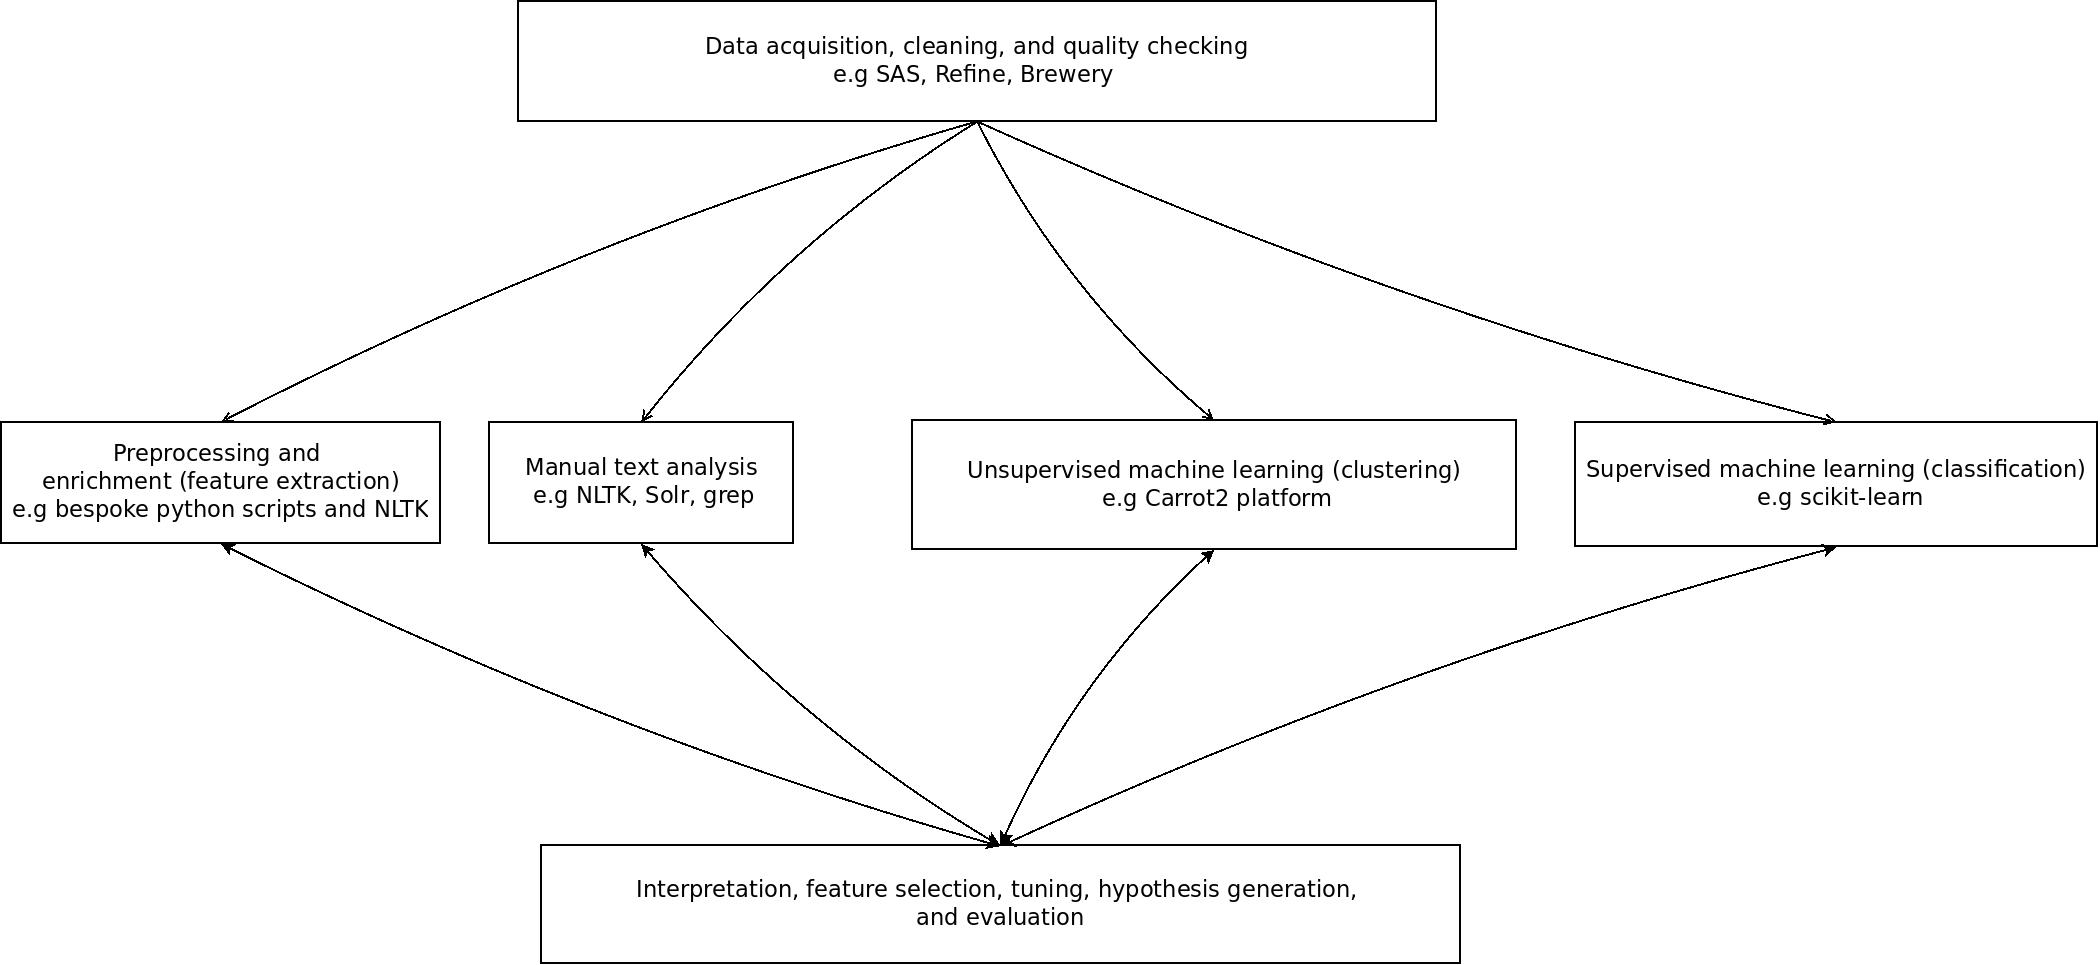
\includegraphics[width=15cm,height=10cm]{figs/DataMiningText3.jpeg}
\caption{Overview of the data mining process with examples of tools used. In addition external corpora may be used to enrich the analysis, and a  visualisation step is usually performed.}\label{fig:dataminingoverview}
\end{figure}


After extraction data were cleaned and selected fields (incident free text description and severity of incident) were converted to csv and xml data formats for subsequent analysis using Apache Solr, Scikit-learn and NLTK (csv), and Carrot2 (xml). Preprocessing techniques including stemming, tokenization, tagging, and filtering were applied. 

Data were audited using Python Brewery and validated by searching for known patterns of interest using grep, Google-refine, and Apache Solr. Data were loaded into NLTK for lexical analysis, Apache Solr to search for strings of interest for validation, the Carrot2 platform for cluster analysis, and Scikit-learn in order to construct a classifier.

Lingo (a clustering algorithm based on the Singular value decomposition) was employed within the Carrot2 platform to perform cluster analysis on selected data for the example problems considered. Naive Bayes (NB) and stochastic gradient descent (SGD) incident severity classifiers were tuned using a grid search strategy and evaluated using cross validation.

\section{Data extraction}

\subsection{Ethics and data storage statement}
This work is an exercise in service development and as such formal ethical approval was not required. Data used have had patient identifiable information removed but are theoretically at risk of deanonymization and so were encrypted and stored in a physically secure location. 

\subsection{The ``computer problem'' extract}

\subsubsection*{SAS Query of NRLS database}
All incidents reported as occurring between 1\ensuremath{^{st}} January 2002 and 1\ensuremath{^{st}} March 2012 and classified as ``Infrastructure (including staffing, facilities, environment)'' (incident category level 1) and ``IT / telecommunications failure / overload'' (incident category level 2), were extracted from the NRLS database using a SAS\textsuperscript{\textregistered} Enterprise Guide 4.3 add-on for Microsoft Office Excel\textsuperscript{\textregistered} on the 20\ensuremath{^{th}} of March 2012.

\section{Data cleaning and audit}
\label{dataqualitymethod}

Ensuring data quality is an essential prerequisite to analysis. Data cleaning and audit methods might help the organisation to identify and monitor data quality issues (see section \ref{howdmhelps}).


The source data for ``computer problem'' extract are incident reports which are completed by individual health care professionals and submitted electronically. Duplicate report submission and submission of reports with missing data is possible and it was therefore important to deduplicate the data and establish its quality. Google-refine\cite{huynhgoogle} (now Open-refine) is a power tool for rapidly cleaning and transforming data and keeping a log of changes made. I chose to use it because it has an easy to use interface and I'm familiar with it. Python Brewery (now Python Bubbles) is a framework for data processing and data quality measurement which makes it easy to rapidly perform tasks such as calculating percentage field completeness for fields in a data table. I chose to use it because I shared a room with the author at EuroPython 2012, he explained the project to me and it seemed to fit with the task.


\subsection{Deduplication and reconciliation}
Google-refine\cite{huynhgoogle} was used to remove duplicates by faceting on the incident description free text field (IN07). Reconciliation was not carried out for time reasons although Google-refine\cite{huynhgoogle} does support this. This would have been helpful for correcting spellings and handling acronyms and synonyms.

\subsection{Python Brewery}
Google-refine\cite{huynhgoogle} was used to establish median field length and number of words per field using the Google Refine Expression Language (GREL). The Python Brewery\cite{pythonbrewery} module was used to calculate field completeness for the data set (see section \ref{brewery_script.py} for source code and \ref{dataqualityresults} for results).


%\begin{minted}{python}
import brewery
from sys import argv

script, inputfilename = argv

b = brewery.create_builder()
b.csv_source("%s" % inputfilename)
b.audit()

b.pretty_printer()

b.stream.run()
\end{minted}

\begin{minted}{python}
#Adapted from code examples in S. Bird, E. Klein, and E. Loper. 
#Natural language processing with Python. O’Reilly Media, 2009
#
#Takes a text file and tokenizes it words, converts to lower lase, filters stop words, 
#builds vocab for text, calculates lexical diversity, builds collocation, builds frequency 
#distribtion of most common words, builds example dispersion plot of words of interest 
#(manually entered below in this script), then displays results 

import nltk
from nltk.corpus import stopwords
from sys import argv

script, inputfilename = argv #takes whatever filename you pass in

print inputfilename

raw = open("%s" % inputfilename).read() #loads incident descriptions identified as being due to computer problems

tokens = nltk.wordpunct_tokenize(raw) #tokenizes free text

#tokens = [nltk.PorterStemmer().stem(t) for t in tokens] 
# uncomment to stem tokens

#tokens = [nltk.WordNetLemmatizer().lemmatize(t) for t in tokens]
# uncomment to lemmatize tokens

text = nltk.Text(tokens) #defines text

words = [w.lower() for w in text] #defines words and makes all words lower case

filtered_words = [w for w in words if not w in stopwords.words('english')] #removes commonly occuring words ("stop words")

vocab = sorted(set(words)) #defines vocabulary

def lexical_diversity(text): #calculate lexical diversity
    return len(text) / len(set(words))

print "the number of words in the text is %d" % len(text)

print "the number of words in the vocabulary is %d" % len(vocab) 

print "lexical diversity is %d" % lexical_diversity(text) #prints lexical diversity

text.collocations() #builds collocations

fdist = nltk.FreqDist(filtered_words)

fdist.plot(50, cumulative=True) #prints a cumulative frequency distribution of the 50 most commonly used words in the text

text.dispersion_plot(["computer", "system", "crash", "bleep", "patient"]) #example dispersion plot using arbitary seach terms
\end{minted}




\section{Exploring the data}
\label{themesmethod}
Tools to explore the data might help to identify novel themes and support analysis of incidents (see section \ref{howdmhelps}).

Grep, Apache Solr, and NLTK, were used to rapidly search for the presence of words suspected to be key words on the basis of the literature review and prior experience (see section \ref{litreviewthemes} for background and \ref{themesresults} for results). Returned incident descriptions were then briefly reviewed in order to get a feel for the types of descriptions contained in the dataset. Finally the Carrot2 platform was used to perform unsupervised clustering of the data. 

\subsection{Grep}
GNU Grep version 2.10, a command-line utility that searches a file for, and returns lines containing, a user specified pattern, was used to search for the presence of incident reports containing words suspected to be key words in computer problems such as ``crashed'', ``locked'', ``froze'' etc. The tool was chosen because the author is familiar with it and it fit well with the task.

\subsection{Apache Solr}
Apache Solr 3.6.0\cite{solr}, an open source search platform, was configured to run locally and used to search incidents for key words (described in section ~\ref{litreviewthemes}) around themes identified from experience including:

\begin{itemize}
 \item Software bugs
 \item Poor reliability
 \item Ongoing problems
\end{itemize}

The platform was chosen because of its powerful full text search capabilities as well as its standard open interface which permitted results to be returned in an xml format that could be fed into the Carrot2 clustering tool used in later analysis.

\subsection{NLTK}
\label{lexicalanalysismethod}
NLTK (version 2.0b9), is a computational linguistic tool for Python. The tool was chosen because the author has some prior knowledge of Python, because it is very well documented, and because it has a strong and supportive online community.  NLTK was used to characterise and explore the text corpus formed by the free text incident descriptions relating to computer problems and to investigate interesting language snippets found.

\subsubsection{Lexical analysis}
Specifically, the name of a text file is passed as an argument to a Python script that reads a string from the text file and divides, or tokenizes, it into a list of substrings. Exactly how depends on the tokenizer used. I used wordpunct tokenize, the standard tokenizer for words and punctuation provided in the NLTK library. As an example, tokenizing the string ``Hello, world.'' with wordpunct tokenize would result in the following list of substrings:

\begin{pyverbatim}
['Hello', ',', 'world', '.']
\end{pyverbatim}

After tokenization the words were all converted to lower case to create a vocabulary and calculate lexical diversity (the number of unique words / the number of words). A set of collocations for the text is then built. A collocation is a sequence of words that occur together unusually often. Thus, 'red wine' is a collocation, whereas 'the wine' is not. Collocations are resistant to substitution, for example, “maroon wine” would sound very odd. They tend to be specific to a given text and so can convey useful information. 

A cumulative frequency distribution plot of the 50 most common words and a text dispersion plot of words of interest, such as those known to be associated with computer failure like ``crash'', was made for interest. A text dispersion plot is a plot of the frequency of occurrences of a word over time (for commented source code see section \ref{lexical_analysis.py}, for code output see section \ref{lexicalanalysisresults}).

%\subsubsection{Collocations}
%\Glspl{collocation} were identified with NLTK using the standard collocation function \Gls{pointwise mutual information} trigrams were also calculated and those occurring less than 10 times were filtered.




\subsubsection{Named entity recognition}
Named entity recognition is used to identify persons, companies, and locations, and discover relationships between them. This was carried out for the text in the following way. Using NLTK, free text descriptions of incident reports were tokenized to sentences and then words, tagged with a POS (part of speech) tagger, and 'chunked' into noun phrases (see figure \ref{fig:elephant}). 'Chunking' means extracting a list of 'chunks', in this case noun phrases, from the text (for commented source code see section \ref{mrchunk.py}).


% add POS labelling and NP chunking code


\begin{figure}[htp]	
\centering
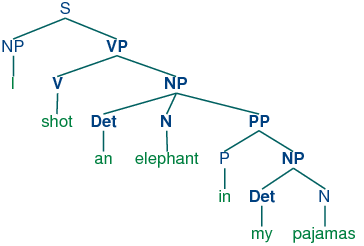
\includegraphics[width=15cm,height=10cm]{figs/elephant.png}
\caption{Example of part of speech tagging in NLTK for an ambiguous phrase. NNP = proper noun, V = verb, Det = determiner, N = noun, P = preposition, VP = verb phrase, NP = noun phrase.}\label{fig:elephant}
\end{figure}

\subsubsection{Investigation of language snippets of interest}
Where snippets of interest, for example ``Computers unable'', which was identified as a cluster using the Carrot2 clustering platform, were found (see figure \ref{fig:lingoclustering}) this was investigated further by review of incidents containing the phrase, identified using grep and/or the Solr search engine and the use of NLTK to, for example, create a frequency distribution plot of the top 50 words which follow ``unable to'' in the text (for commented source code see section \ref{unable_analysis.py} and for results see section \ref{unabletosnippetsresults}).


\section{Lingo}
\label{lingomethod}
% Lingo\cite{Osiriski2004} is a search results clustering algorithm that is part of the Carrot 2 platform \cite{Osinski2005}. The Carrot 2 platform is a piece of open source java software that facilitates application of the Lingo algorithm to appropriately formatted locally stored data.
Clustering is an unsupervised machine learning technique (see section \ref{clusteringintro}) that might support human analysis of large numbers of patient safety incidents (see section \ref{howdmhelps})

The lingo algorithm was chosen because it seems to map well to the domain problem considered. It is typically used for search engine result clustering so for example a search for apache would return semantically usefully labelled clusters of results e.g  ``Apache Indians, ``Apache helicopters'', ``Apache Software Foundation'', ``Apache Licence'',  ``Apache Wars'' etc. The group of incidents considered in this dissertation are in a sense ``search results'' to be summarised since they were obtained by searching the NPSA database for all incidents classified as being to with computer problems. The algorithm was also applied to search results for searches within the sample, produced using the Solr search engine, for strings of interest.

The algorithm is based on \gls{Singular Value Decomposition}(SVD) and uses a \gls{Vector Space Model}(VSM) with each document \textit{d} being represented as a \textit{document vector} \ensuremath{[\omega_{t_{0}},\omega_{t_{1}},\dotsc \omega_{t_{\Omega}}]} where \ensuremath{t_{0},t_{1},\dotsc t_{\Omega}} is a set of words and \ensuremath{\omega_{t_{i}}} expresses the weight (importance) of term \ensuremath{t_{i}} to document \textit{d} and each term is assumed to be an independent dimension. Collections of \textit{document vectors} form a \textit{term-document matrix}, with the value of each element depending on the strength of association with the respective document. Singular value decomposition, a way of factorizing the matrix, is then used  to find clusters.

There are three phases to clustering with the lingo algorithm:
		  \begin{enumerate}
                     \item Cluster discovery (unsupervised phrase extraction)
		      \item Candidate label discovery (cluster-label-induction)
		      \item Cluster-label matching (cluster-content allocation)
                    \end{enumerate}
                    

The phrase extraction phase discover phrases and single terms that could potentially explain the verbal meanings of SVD-derived abstract concepts using a modified semantic hierarchical clustering (SHOC) algorithm. 
  
The cluster-label-induction phase identifies the abstract concepts that best describe the input document collection and uses frequent phrases to construct a human-readable representation of these concepts (the cluster labels).

Cluster labels are required to:\begin{itemize}                                                                                                                                                                                                                                              									\item appear in the input snippet at least a specified number of times
									  \item not cross sentence boundaries
									  \item be as complete as possible
									  \item neither begin nor end with a stop word
									\end{itemize}

Finally, in the cluster-content allocation phase input documents are matched against cluster labels, if the similarity exceeds a predefined threshold then the document is allocated to the cluster. 

To use the Carrot2 platform it was necessary to convert the .csv file into an appropriately formatted .xml file. This was achieved using a python script that Ross Jones helped me to write (for commented source code see section \ref{csv2xml.py} and for results see section \ref{lingoresults}).


\section{Scikit-learn}
\label{classificationmethod}

Classification is a supervised machine learning technique (see section \ref{classificationintro}) that might help to ensure the accuracy of the classification of the severity of patient safety incidents (see section \ref{howdmhelps}).

Scikit-learn is is an open source machine learning library for the Python programming language. It supports supervised text classification tasks using Naive Bayes (NB) and Stochastic Gradient Descent (SGD) algorithms. I used it because Python is my preferred programming language and because Scikit-learn is a very well documented project with a large and very supportive community. 

\subsection{Classification task}
The example classification task chosen was to classify the degree of harm of a clinical incident based on its description.\

The training data set was composed of incident description and degree of harm fields. Each incident has an incident description and a human-assigned degree of harm category.

Categories used are:\begin{itemize}
                      \item Death
		      \item Severe
		      \item Moderate
		      \item Low
		      \item No Harm
                     \end{itemize}

\subsection{Adapting the 20 Newsgroups data set code examples}
The 20 Newsgroups data set (see section \ref{twentynews} also) is a collection of approximately 20,000 newsgroup documents, partitioned (nearly) evenly across 20 different newsgroups. It is a very popular data set for testing text classification applications and there existed many examples for scikit-learn. The standard classification task considered is to predict the newsgroup that the document belongs to on the basis of the document contents. This is roughly analogous to predicting severity based on document contents so I decided to adapt these examples for my purposes by converting my patient safety data set into a similar format to the 20 Newsgroups data set and editing the code as necessary.

\subsubsection{Splitting the patient safety dataset into training and testing subsets}
To avoid the problem of overfitting it was necessary to split the original data set into training and testing subsets. This is achieved using a Python script (incidentsplit.py) and with the csv and numpy libraries to read the original csv and split it into a training dataset (2/3) and a testing dataset (1/3) in a randomised fashion (for commented source code see section \ref{incidentsplit.py}).


\subsubsection{Extracting incidents and placing them in a folder structure}
Messages in the 20 newsgroups data set are arranged in 20 folders which are labelled according to the name of the newsgroup the message was posted to. To prepare my dataset for analysis it was necessary to extract incidents and place them into folders labelled according to the severity of the incident.  This was achieved using a Python script (incidentextract.py) that reads a csv file and writes the free text incident description into a folder that matches its severity category (for commented source code see section \ref{incidentextract.py}).


\subsubsection{Selecting a classifier}
Different classifiers were evaluated by adapting an existing 20 newsgroup scikit-learn Python classifier comparison script to use the computer incident data (for commented source code see section \ref{classifierselection.py}). As part of this process the effect of tuning classifier parameters, weightings, balancing the data set, and simplifying the task to a binary (death OR severe) vs not(death OR severe) classification were examined. Two classifiers, MultinomialNB and SGDClassifier appeared to perform particularly well and were selected for further optimization. To experiment with balancing the training data set all deaths and severe incidents (N=51) were used as positives and matched with a random selection of 51 incidents from the pool of all incidents that weren't death or severe incidents (for commented source code see section \ref{randomselect.py}).


\subsubsection{Classification}
Training and test datasets are loaded into scikit-learn from a folder container which contains two subfolders 'Training' and 'Testing'. Within each subfolder there are five further subfolders 'Death', 'Severe', Moderate', 'Low', 'No Harm' containing the appropriate free text incidents as individual files (for commented source code see section \ref{incident_classify.py}).

Countvectorizer converts the collection of text documents into a matrix of token counts. The default setting of word tokenisation is used. 

Term occurrences (X\_counts) fails to take account of document size. Longer documents may have higher average count values than shorter ones even though they talk about the same topic. To avoid this the number of occurrences in any document is divided by the total number of words in that document to give the Term Frequency (tf) using the function TfidfTransformer. 

The MultinomialNB function is used to implement a multinomial Naive Bayes classifier which is suitable for classification tasks involving data with discrete features (i.e the word counts we have generated for text classification). SGDClassifier, uses a Stochastic Gradient Descent algorithm which is an efficient learning algorithm for large text data sets and supports sample weighting. SGDClassifier was also chosen because it has performed well in recent public online text classification challenges hosted by the machine learning challenge website kaggle.com (see section \ref{twentynews} also).

Parameters for MultinomialNB and SGDClassifier were optimized using a the scikit learn grid search and pipe libraries which allow automated parameter tuning and evaluation to optimise algorithm performance (for commented source code see section \ref{gridsearch.py} and for results see section \ref{classificationresults}).

Classifier performance was measured by cross validation. The dataset is split into training and testing partitions in a ratio of 2:1. The model is trained on 2/3rds of the labelled data, the training set, and tested against the remaining 1/3rd of the data, the testing set. Partitions are created by random sampling of the dataset. In this way training the classifier on the testing dataset and the resultant problem of overfitting are avoided.




%could add a word list
%could add code and results

